\subsection{Hardware}

The SparrowE wireless sensor nodes are custom designed for use in various research projects.
They are designed as a single PCB board which hosts all of the major components, such as: controller,
RF module, power supply and sensors. The main the main processing unit of the SparrowE nodes is an Atmel 
ZigBit 900MHZ RF module\cite{AtmelZigBit900}, which hosts both the microcontroller, an ATmega 1281V 8-bit microcontroller \cite{ATmega1281} and the 
wireless transceiver, an AT86RF212 RF chip \cite{AT86RF212}. These two components are connected via an SPI line inside the ZigBit 
module. The 8 bit, low power, Atmega 1281V microcontroller is connected to all of the node's sensors and its 
main function is to process the data received from them and pass it on to the RF transceiver. The AT86RF212 RF 
is a low power wireless transmission chip capable of sending signals to distances of up to a few kilometers, according 
to the official datasheet \cite{datasheetatmel}. It also provides an AES-128 compatible security module for data 
encryption and decryption.

\begin{figure}[ht] \centering
  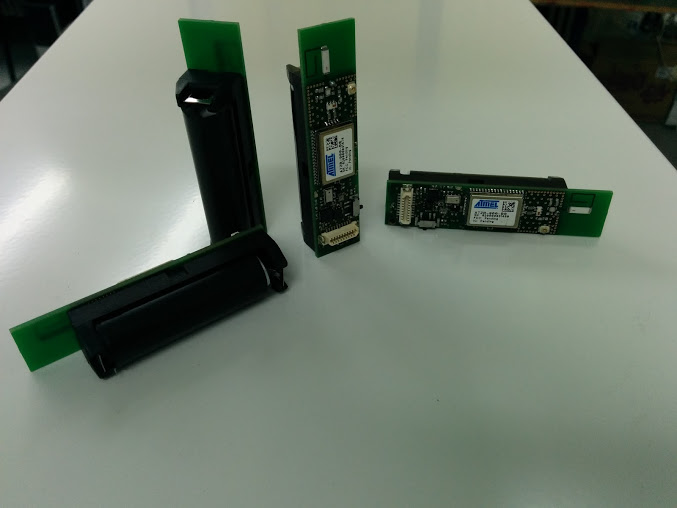
\includegraphics[width=0.45\textwidth]{img/sparrow-nodes.jpg}
  \caption{SparrowE wireless sensor nodes}
\end{figure}

In order to monitor its environment, the SparrowE wireless sensor node relies on 3 main sensor peripherals. The first is 
an Si7020 humidity and temperature sensor\cite{Si7020} with incorporated ADC unit. The measurement resolution for relative humidity measurements
can vary between 8 and 12 bits, while the resolution for temperature measurements varies from 11 to 14 bits. The second sensor is 
an MPL3115A2 \cite{MPL3115A2} altimeter which can measure pressure and altitude. This sensor also has an incorporated ADC unit and can measure 
both altitude and pressure with a precision of up to 20 bits. The final sensor mounted on the SparrowE and the most important for 
earthquake and vibration monitoring is the LSM9DS0 IMU(Inertial Measurement Unit)\cite{LSM9DS0}. This chip has 3 channels for linear acceleration measurement, 
3 channels for angular rate measurement and another 3 channels for magnetic field measurement. All data measurements are performed at a 
16 bit resolution. From this last sensor, the metric used by the presented application is the linear acceleration (measured in Gs).
All of the aforementioned sensors are connected to the microcontroller via a two-wire interface. Each of the has a different slave address so 
it is possible for the master, the Atmega 1281V controller, to communicate with all of them without interference from the others.

\begin{figure}[ht] \centering
  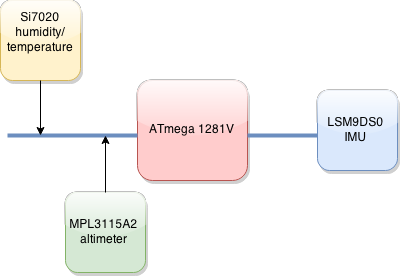
\includegraphics[width=0.5\textwidth]{img/i2c-connection.png}
  \caption{Sensors connected on two-wire interface}
\end{figure}

All the components on the SparrowE node function at a maximum supply voltage of 3.6V. The node can be powered in 2 ways: either from a lithium polymer battery 
cell or via an USB port. When powered via USB, a linear DC regulator is used to drop the supply voltage from the 5V of the USB line to the necessary 3.3V.

\subsection{Software}

The SparrowE wireless sensor nodes run an Arduino\cite{arduino} compatible firmware. This allows the programmer to easily import 
and use open source Arduino modules for each peripheral. Another advantage of using an Arduino compatible firmware is that it ensures the code is 
compatible with multiple platforms and can be easily modified, upgraded or ported to similar hardware. For development, the Arduino IDE is used 
because it provides access to predefined libraries for peripherals such as serial line, two-wire interface and ADC. It is also available on a wide 
variety of operating systems which makes code modifications and firmware updates easier to implement.

The firmware which runs on the SparrowE nodes operates in two steps. The first step is a calibration phase, which starts running when the sensor 
is first turned on. This will determine the default values for each of the 3 accelerometer axes for the current position of the node. Once this step 
is completed, the node enters its second step in which it will continuously function untill it is turned off. During this period, it harvests data 
from the accelerometer and sends it towards a designated gateway using the AT86RF212 RF transceiver. The gateway shall always be connected to a server 
which is capable of plotting and analyzing the data. The gateway communicates with this server by means of a serial interface.

\begin{figure}[ht] \centering
  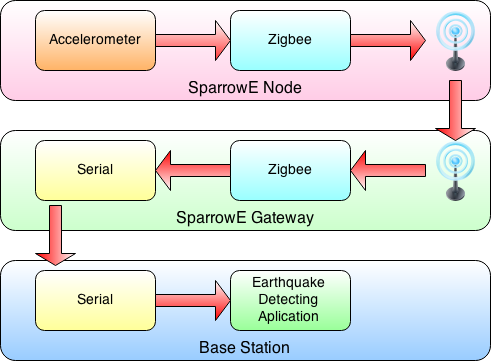
\includegraphics[width=0.5\textwidth]{img/software-architecture.png}
  \caption{Software arhitecture connections}
\end{figure}

The accelerometer on the SparrowE node is configured for a +/-2G linear acceleration rate and operates at an Ouput Data Rate of 50 Hz. 
The raw data from the 3 axes is translated by the Atmega 1281V microcontroller into gravitational scale and then is normalized using the following formula:

$ a = \sqrt{x^2+y^2+z^2}$

This approach will generate a value of 1G when the node is kept still, in its calibrated position. When the surface starts vibrating, the value will start varying 
above or bellow the refence value of 1G. The calculated data is gathered in arrays containing 20 samples each. They are sent periodically by the transceiver to the 
gateway. Node identification data is also added to the sent packets. The gateway is able to collect data from multiple nodes and send it to the base station through
the aforementioned serial connection, which is configured at a baud rate of 1Mbps. The base station is responsible for saving and interpreting the data. 
It is considered that a node has detected an earquake if the values oscilate strongly around the 1G reference value.


\subsection{Low Power}

Since the goal of the sensors is to monitor phenomena which does not frequently occur in many areas, we must ensure that the SparrowE sensors are low power and 
capable of running for prolonged periods of time. This problem is tackled mainly at the software level. At the hardware level, while the components of the sensor 
are selected with regard to power consumption, their power consumption is still too much considering the target autonomy of the SparrowE sensor.

In order to overcome this, the firmware is designed to keep the controller in a sleep state and wake up periodically to read the accelerometer data. 
The gating is done using a RTC (Real Time Clock). The AtmegRFA1 controller on the sensors offers the ability of using Timer2 as a real time clock source with an 
external 32Mhz crystal oscilator. The reason why a real time clock is used to implement this mechanism is that even while the controller sleeping, 
this peripheral is still active and it will generate interrupts at certain time intervals configured by the programmer. When the controller receives such an 
interrupt, it will wake up and perform any designated operation until it is put back to sleep and the entire process starts again.

By using this technique, the data from the accelerometer is read and sent to a base station once every second instead of once every hundreds of miliseconds. By doing this, 
the battery is preserved for much longer, as the controller and the transceiver operate for smaller periods of time. The risk of losing data from the accelerometer is reduced 
because older readings are kept in a small buffer. Thus, when performing a read, we get the values of the accelerometer's most recent X reads, instead of just one read. Also, 
in time, the data loses continuity as we are getting discrete values for moments in time set 1 second apart instead of a continuous flow, but it is easier to identify when 
a transition from no vibrations to actual vibrations occur.

With this approach, we increase the autonomy of the Sparrow sensors while, at the same time, making data easier to handle by the plotting and interpretation software running 
on the base station.
